\documentclass[slovene,11pt,a4paper]{article}
%\usepackage{fullpage}
\usepackage[margin=2cm]{geometry}

\usepackage[T1]{fontenc}



%dodatni paketki:
\usepackage{graphicx}
\usepackage{amsmath,amsfonts,amsthm} %matematicni paket
\usepackage{color} % omogoča barvno pisanje
\usepackage[utf8]
{inputenc}
\usepackage[slovene]{babel} % slovenski jezik/hyphenation
\usepackage{hyperref} %naredi vse povezave rečerenc, kazala,...
\numberwithin{equation}{section} % Number equations within sections (i.e. 1.1, 1.2, 2.1, 2.2 instead of 1, 2, 3, 4)
\numberwithin{figure}{section} % Number figures within sections (i.e. 1.1, 1.2, 2.1, 2.2 instead of 1, 2, 3, 4)
\numberwithin{table}{section} % Number tables within sections (i.e. 1.1, 1.2, 2.1, 2.2 instead of 1, 2, 3, 4)
\usepackage{eurosym} %za znak €

\usepackage{mathrsfs}
\usepackage{mathabx} % za kemisjke smeri in naslednje 3 vstrice
\catcode`_=12
\begingroup\lccode`~=`_\lowercase{\endgroup\let~\sb}
\mathcode`_="8000


\usepackage[margin=2cm]{geometry}



\begin{document}
\begin{titlepage}

\newcommand{\HRule}{\rule{\linewidth}{0.5mm}} % Defines a new command for the horizontal lines, change thickness here

\center % Center everything on the page

%----------------------------------------------------------------------------------------
%	LOGO
%----------------------------------------------------------------------------------------

%\includegraphics{Logo}\\[1cm] % Include a department/university logo - this will require the graphicx package
 
%----------------------------------------------------------------------------------------


\includegraphics[width=2cm]{slike/aaa}\\[0.5cm]
 
%----------------------------------------------------------------------------------------
%	NASLOV DELA
%----------------------------------------------------------------------------------------
\textit{Univerza v Ljubljani}\\
\textit{Fakulteta za {\color{red}matematiko in fiziko}}\\[0.5cm]

\emph{Oddelek za fiziko}\\[0.5cm] % Oddelek za fiziko


%----------------------------------------------------------------------------------------
%	TITLE SECTION
%--------------------------------------------------------------------------------------
\HRule \\[0.4cm]
\huge {\bfseries 7. naloga: - Razdelčni in nelinearni modeli}\\[0.4cm] % NASLOV SEMINARJA
\HRule \\[0.5cm] 

 \textsc{\large Poročilo pri predmetu modelska analiza 1}\\
 \textsc{\large 2015/2016}\\[1cm] % SEMINASKO DELO
 
%----------------------------------------------------------------------------------------
%	AUTHOR SECTION
%----------------------------------------------------------------------------------------



% If you don't want a supervisor, uncomment the two lines below and remove the section above
\Large \emph{Avtor:}\\
Klemen \textsc{Rahne}\\
28152028\\[2cm]
%----------------------------------------------------------------------------------------
%	DATUM
%----------------------------------------------------------------------------------------

{\large \today } \\[0.5cm] % Date, change the \today to a set date if you want to be precise

	

\end{titlepage}


%----------------------------------------------------------------------------------------
%	KAZALO
%----------------------------------------------------------------------------------------

%\tableofcontents

%----------------------------------------------------------------------------------------
%	ZAČETEK TEKSTA
%----------------------------------------------------------------------------------------

\section{Farmakološki model}
Tako kot v prejšnji nalogi imamo farmakološki model z enakimi podatki. Sedanji model, odziv tkiva $y$ v odvisnosti od vnesene doze reagenta, opisujemo s tremi parametri $p$, $a$ in $y_0$:
\begin{equation}
\label{farmacevti-1}
y=\frac{y_0 x^p}{x^p+a^p}
\end{equation}
\subsection{Primerjava z linearnim prilagajanjem}
V prejšnji nalogi smo imeli vrednost parametra $p=1$, ter smo enačbo preoblikovali v linearno obliko, ter jo nato prilagajali linearno. Primerjajmo vrednosti parametrov med linearnim in nelinearnim prilagajanjem.

\begin{table}[h]
\centering
\label{tabela-1}
\begin{tabular}{l|l|l|l|l|}
\cline{2-5}
                             & \multicolumn{2}{l|}{linearno prilagajanje} & \multicolumn{2}{l|}{linearno prilagajanje} \\ \cline{2-5} 
                             & vrednost             & napaka              & vrednost             & napaka              \\ \hline
\multicolumn{1}{|l|}{$y_0$}  & 104.8                & $\pm$2.5            & 106.3                & $\pm$4.6            \\ \hline
\multicolumn{1}{|l|}{a}      & 21.2                 & $\pm$1.3            & 24.7                 & $\pm$3.8            \\ \hline
\multicolumn{1}{|l|}{$\chi^2$} & 26.08                &                     & 22.01                &                     \\ \hline
\end{tabular}
\end{table}

\begin{figure}[h]
\centering
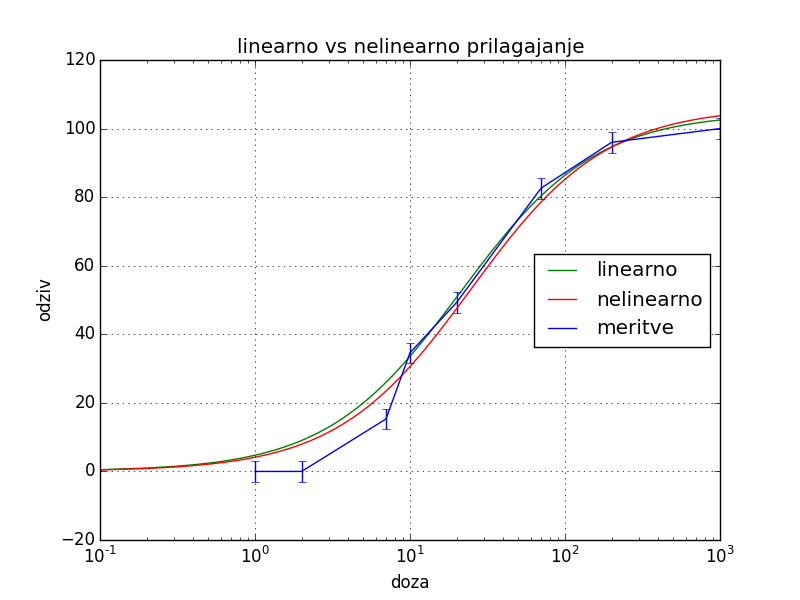
\includegraphics[scale=0.6]{slike/primerjava-line-nelinearno.png}
\caption[farmacevt-lin-vs-nelin]{Primerjava med linearnim in nelinearnim prilagajanjem.}
\label{fig:prva-1}
\end{figure}
Pričakovali bi, da bosta oba prilagajanja enak, vendar iz vrednosti $\chi ^2$ ugotovimo, da je nelinearno prilagajanje nekoliko boljše.

\subsection{Parameter p}
Oglejmo si, kako dobro prilagajanje dosežemo s prilagajanjem prvotne enačbe \ref{farmacevti-1}.
\begin{table}[h]
\centering
\label{my-label}
\begin{tabular}{l|l|l|}
\cline{2-3}
                               & vrednost & napaka    \\ \hline
\multicolumn{1}{|l|}{p}        & 1.36     & $\pm$0.17 \\ \hline
\multicolumn{1}{|l|}{$y_0$}    & 99.6     & $\pm$3.5  \\ \hline
\multicolumn{1}{|l|}{a}        & 19.8     & $\pm$2.3  \\ \hline
\multicolumn{1}{|l|}{$\chi^2$} & 9.36     &           \\ \hline
\end{tabular}
\end{table}


\begin{figure}[h]
\centering
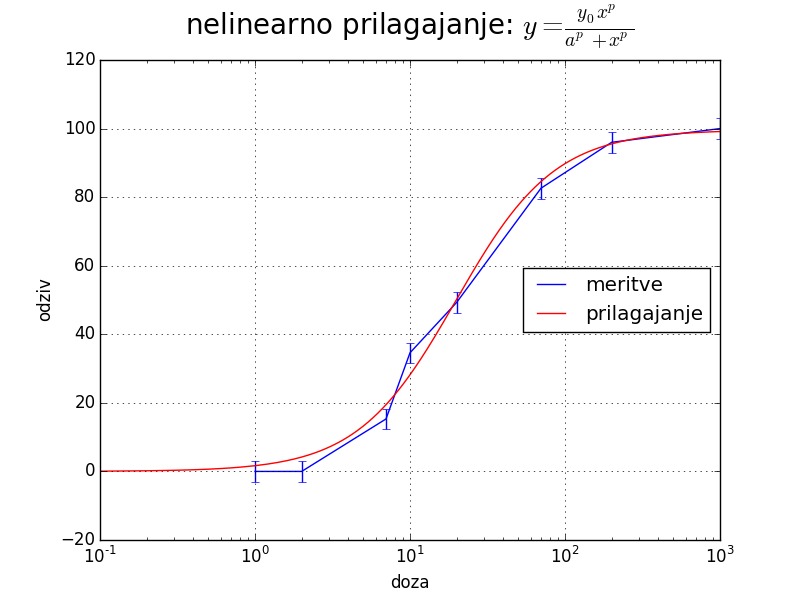
\includegraphics[scale=0.7]{slike/dodatno_parameter.png}
\caption[farmacevt-dodatni-parameter]{Prilagajanje z vpeljavo dodatnega parametra $p$.}
\label{fig:prva-2}
\end{figure}
Z vpeljavi dodatnega parametra, izboljšamo prilagajanje, saj vrednost $\chi^2$ pade za $1/2$ v primerjavi z le dvema parametroma.

\section{Čiščenje ledvic}
Oglejmo si model čiščenja ledvic. V telesu se zadržujejo odpadne snovi, ki se preko ledvic izločajo iz telesa. S pomočjo radioaktivnega sledilca izmerimo časovni potek koncentracije odpadnih snovi v telesu. Iz meritev določimo posamezne parametre, ki nam povedo v kakšnem stanju so ledvica.

\subsection{Enorazdelčni model}
V naših ledvicah predpostavimo, da je hitrost izločanja odpadnih snovi odvisna od pretoka krvi skozi ledvica $\Phi$, koncentracije odpadnih snovi $c$, volumna ledvic $V$ ter učinkovitostjo prečiščevanja $\epsilon$
\begin{equation}
\dot{c}=-\frac{\epsilon \Phi}{V} c
\end{equation}
Rešitev zgornje enačbe je preprosta eksponentna padajoča funkcija:
\begin{equation}
c=c_0 e^{- \lambda t}
\end{equation}
Vemo, da je v krvi koncentracija odpadnih snovi sorazmerna koncentraciji radioaktivnega sledilca, zato lahko zgornjo enačbo prevzamemo na število razpadov sledilca:
\begin{equation}
N=N_0 e^{- \lambda t}
\end{equation}
Iz jedrskega razpada vemo, da je standardni odklon enak korenu vseh detektiranih razpadov v danem času:
\begin{equation*}
\sigma_{N_i}=\sqrt{N_i}
\end{equation*}
Najprej poglejmo, kako dobro se prilagaja zgornji model.
\begin{figure}[h]
\centering
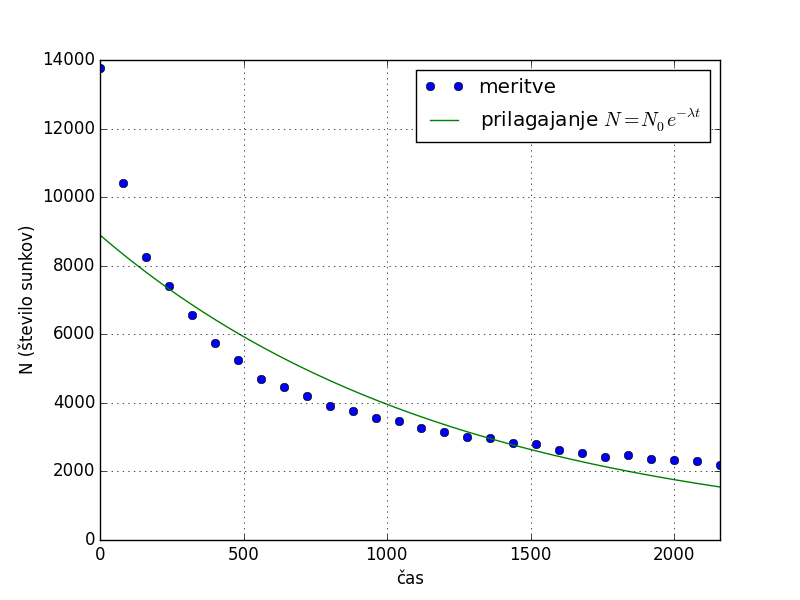
\includegraphics[scale=0.55]{slike/druga_najosnovna.png}
\caption[farmacevt-dodatni-parameter]{nelinearno prilagajanje krivulji $N=N_0 e^{-\lambda t}$.}
\label{fig:druga-1}
\end{figure}
Optimalna parametra pri zgornjem modelu sta $N_0=8894.5\pm 549.0$, $\lambda = 8.1 \times 10^{-4}\pm 6.6\times10^{-5}$, vrednost $\chi^2=4058$. Že iz grafa opazimo, da tak model ni najboljši. Zato ga dopolnimo. Če dodatno upoštevamo če konstantno ozadje pade vrednost $\chi^2$ na $521.3$, ter vrednosti parametrov $N_0=9828.6\pm 343.3$, $\lambda = 2.50\times10^{-3}\pm 1.4\times10^{-4}$ ter $B=2438 \pm 82.7$.

\begin{figure}[h]
\centering
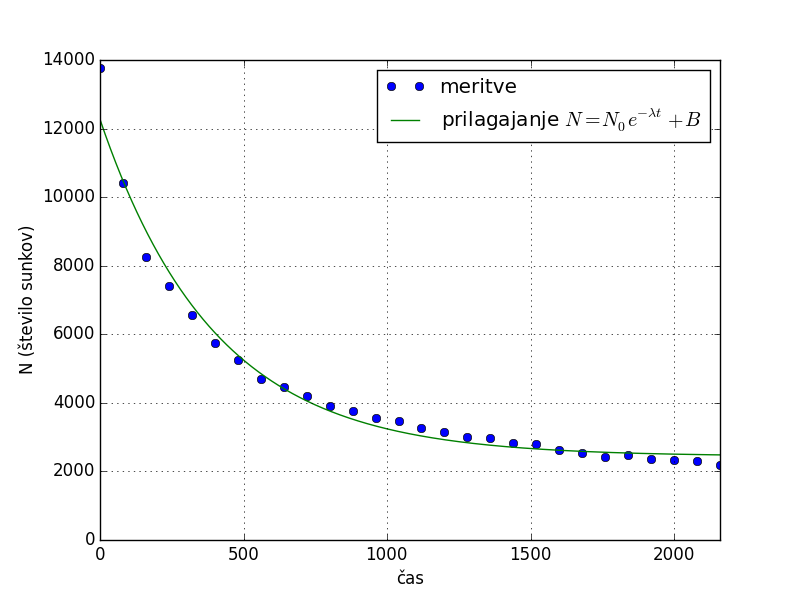
\includegraphics[scale=0.55]{slike/druga.png}
\caption[farmacevt-dodatni-parameter]{nelinearno prilagajanje krivulji $N=N_0 e^{-\lambda t}+B$.}
\label{fig:druga-2}
\end{figure}
\pagebreak


\subsection{Dvorazdelčni model}
Ker so ledvice del večjega sistema (organizma), ledvice interagirajo tudi z ostalimi organi, tkivi. Posledično enorazdelčni opis ni dovolj dober. Zato naš model opišemo z naslednjo funkcijo:
\begin{equation}
\label{dvorazdelčni-1}
N=A e^{- \lambda_1 t} + B e^{- \lambda_2 t}
\end{equation}
Pri prilagajanju te funkcije na podatke dobimo naslednje vrednosti parametrov:
\begin{table}[h]
\begin{center}

\begin{tabular}{l|l|l|}
\cline{2-3}
                                  & vrednost      & napaka           \\ \hline
\multicolumn{1}{|l|}{A}           & $5231.2$      & $\pm170.7$       \\ \hline
\multicolumn{1}{|l|}{$\lambda_1$} & $4.2\times10^{-4}$ & $\pm2.1\times10^{-5}$ \\ \hline
\multicolumn{1}{|l|}{B}           & $8177.1$      & $\pm 66.0$       \\ \hline
\multicolumn{1}{|l|}{$\lambda_2$} & $4.8\times10^{-3}$ & $\pm2.3\times10^{-4}$    \\ \hline
\multicolumn{1}{|l|}{$\chi^2$}    & $72.6$        &                  \\ \hline

\end{tabular}
\end{center}
\end{table}

\begin{figure}[h]
\centering
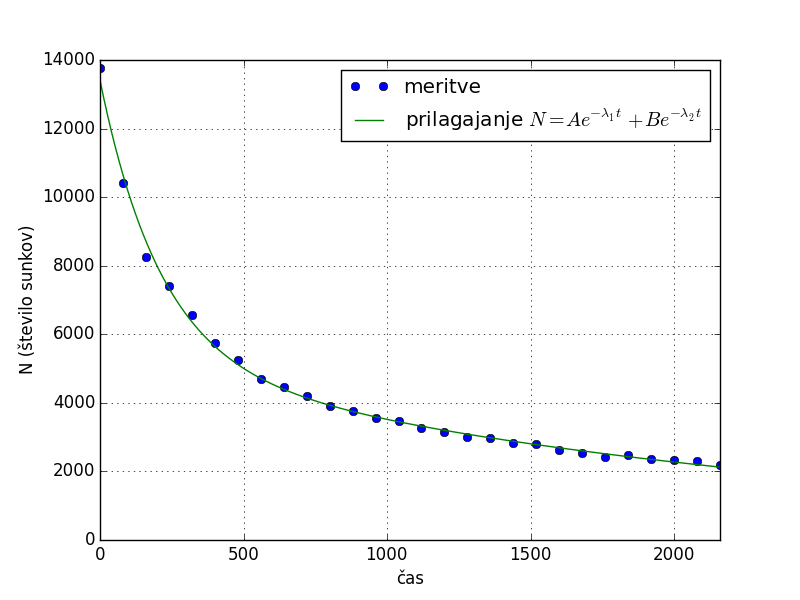
\includegraphics[scale=0.55]{slike/druga_1a.png}
\caption[farmacevt-dodatni-parameter]{nelinearno prilagajanje krivulji $N=A e^{- \lambda_1 t} + B e^{- \lambda_2 t}$.}
\label{fig:druga-3}
\end{figure}
Vrednost $\chi^2$ pade s $521$, na $72.6$, kar je že razlika v enem velikostnem razredu. Zato lahko predpostavimo, da tak dvorazdelčni model bolje opiše delovanje ledvic, kot pa enorazdelčni model.\\
Dodatno si oglejmo še en model delovanja ledvic, v katerega vpeljemo člen $e^{-\lambda \sqrt{t}}$. Torej prilagajamo naslednjo funkcijo:
\begin{equation}
\label{eq-koren}
N=A e^{- \lambda_1 t} + B e^{-\lambda_2 \sqrt{t}}
\end{equation}
Optimalni parametri za zgornjo funkcijo pri danih podatkih so:

\begin{table}[h]
\begin{center}

\begin{tabular}{l|l|l|}
\cline{2-3}
                                  & vrednost           & napaka             \\ \hline
\multicolumn{1}{|l|}{A}           & $4970$             & $\pm286$           \\ \hline
\multicolumn{1}{|l|}{$\lambda_1$} & $4.2\times10^{-3}$ & $\pm1.7\times10^{-4}$ \\ \hline
\multicolumn{1}{|l|}{B}           & $8794.7$           & $\pm322.4$         \\ \hline
\multicolumn{1}{|l|}{$\lambda_2$} & $3.0\times10^{-2}$ & $\pm9.4\times10^{-4}$ \\ \hline
\multicolumn{1}{|l|}{$\chi^2$}    & $29.4$             &                    \\ \hline
\end{tabular}
\end{center}
\end{table}

\begin{figure}[h]
\centering
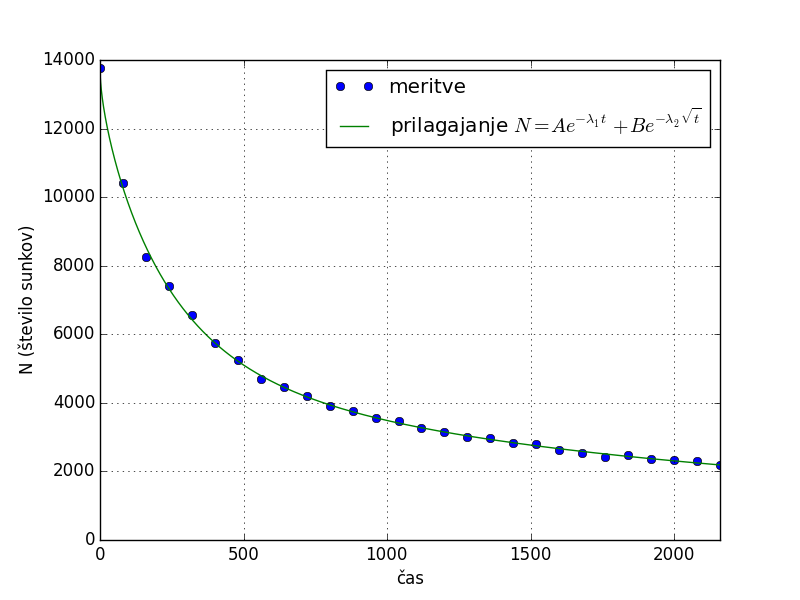
\includegraphics[scale=0.7]{slike/druga_2.png}
\caption[farmacevt-dodatni-parameter]{nelinearno prilagajanje krivulji $N=A e^{- \lambda_1 t} + B e^{- \lambda_2 t}$.}
\label{fig:druga-4}
\end{figure}
\pagebreak
S prostim očesom se razlike med grafoma \ref{fig:druga-3} in \ref{fig:druga-4} ne opazi. Vrednosti $\chi^2$ za omenjena grafa se razlikuje za faktor $\approx2$, v korist modela \ref{eq-koren}. Vsekakor lahko rečemo, da za opis delovanje ledvic bolje opisuje dvorazdelčni opis.

\section{Korozija}
Lastnost korozije, lahko določimo iz parametrov, ki jih določimo iz U-I diagrama med kovino in korozivnim elektrolitom. Osnovni model opisujejo trije parametri $I_0$, $U_a$, $U_b$:
\begin{equation}
\label{eq-korozija-1}
I=I_0\left[\exp\left(\frac{U}{U_a}\right)-\exp\left(-\frac{U}{U_c}\right)\right]\quad
\end{equation}
Za tak model dobimo naslednje vrednosti parametrov:
\begin{table}[h]
\begin{center}
\begin{tabular}{|l|l|l|}
\hline
 & vrednost & napaka \\ \hline
$I_0$ & $2.6\times 10^{-3}$ & $3.9\times 10^{-4}$ \\ \hline
$U_a$ & $138.7$ & $\pm25.1$ \\ \hline
$U_b$ & $74.0$ & $\pm6.9$ \\ \hline
$\sigma^2 \chi^2$ & $4.2\times 10^{-8}$ &  \\ \hline
\end{tabular}
\end{center}
\end{table}

Predpostavljamo, da so pri vseh meritvah toka napake konstantne ($\sigma$), ker pa ne vemo vrednosti, lahko vrednost $\sigma^2 \chi^2$ obravnavamo kot kvaliteto prilagajanja.
\begin{figure}[h]
\noindent\makebox[\textwidth][l]{%
\hspace{-\dimexpr\oddsidemargin+1in}%

\begin{minipage}[t]{0.5\paperwidth}
\begin{flushleft}

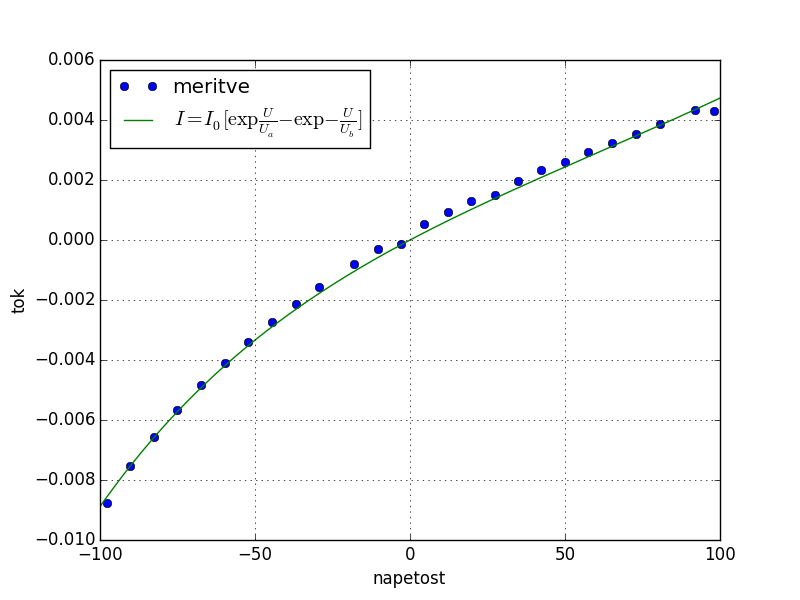
\includegraphics[scale=0.45]{slike/tretja_1.png}
\caption{Nelinearno prilagajanje $I=I_0 [\exp{\frac{U}{U_a}}- \exp{-\frac{U}{U_b}}]$.}
\hspace{\fill}
\end{flushleft}
\end{minipage}
\begin{minipage}[t]{0.5\paperwidth}
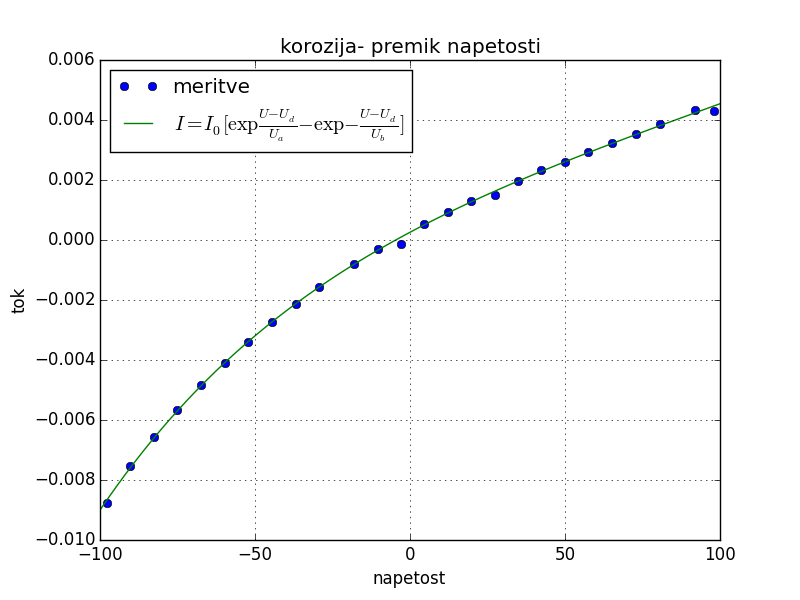
\includegraphics[scale=0.45]{slike/tretja_2.png}
\caption{Nelinearno prilagajanje s premikom napetosti.}
\end{minipage}%
}
\end{figure}
\pagebreak

Poskusimo naš model še bolj izpopolniti. Opazimo, da naše izmerjene točke ne potekajo skozi izhodišče, zato v \ref{eq-korozija-1} vpeljemo linearni premik napetosti: $U \rightarrow U-U_d$:
\begin{equation}
\label{eq-korozija-2}
I=I_0\left[\exp\left(\frac{U-U_d}{U_a}\right)-\exp\left(-\frac{U-U_d}{U_b}\right)\right]\quad
\end{equation}
Pri taki izbiri modelske funkcije se vrednost parametrov nekoliko spremenijo, vrednost $\sigma^2 \chi^2$, pa se zmanjša za en velikostni razred. Torej smo dobili boljšo modelsko funkcijo.

\begin{table}[h]
\begin{center}
\begin{tabular}{|l|l|l|}
\hline
 & vrednost & napaka \\ \hline
$I_0$ & $3.1\times 10^{-3}$ & $\pm2.4\times 10^{-4}$ \\ \hline
$U_a$ & $198.0$ & $\pm24.0$ \\ \hline
$U_b$ & $76.6$ & $\pm3.5$ \\ \hline
$U_d$ & $-4.61$ & $\pm0.42$ \\ \hline
$\sigma^2 \chi^2$ & $5.76\times 10^{-9}$ &  \\ \hline
\end{tabular}
\end{center}
\end{table}



\subsection{Taylorjev razvoj/linearni problem}
Naše izmerjene točke lahko tudi prilagodimo polinomu $n$-te stopnje. Zaradi relativno majhne ukrivljenosti bomo prilagajali polinom tretje stopnje:
\begin{equation}
\label{korozija-taylor1}
I=A+B U+C U^2+D U^3
\end{equation}
Optimalni parametri so:

\begin{table}[h]
\begin{center}
\begin{tabular}{|l|l|l|}
\hline
 & vrednost & napaka \\ \hline
$A$ & $2.92\times 10^{-4}$ & $\pm3.0\times 10^{-5}$ \\ \hline
$B$ & $5.51\times 10^{-5}$ & $\pm8.4\times 10^{-7}$ \\ \hline
$C$ & $-2.44\times 10^{-7}$ & $\pm6.5\times 10^{-9}$ \\ \hline
$D$ & $1.24\times 10^{-9}$ & $\pm1.2\times 10^{-10}$ \\ \hline
$\sigma^2 \chi^2$ & $7.58\times 10^{-9}$ &  \\ \hline
\end{tabular}
\end{center}
\end{table}
Opazimo, da vrednosti koeficientov, ki pripadajo posamezni stopnji padajo z naraščanjem stopnje. To opravičuje našo linearizacijo. Tudi vrednost $\sigma^2 \chi^2$ je primerljiva z vrednostjo, ko smo eksaktno prilagajali z odmikom napetosti. Če želimo določiti parametre $U_a$, $U_b$, $U_d$ ter $I_0$, je potrebno enačbo \ref{eq-korozija-2} razvito po Taylorju, ter nato vzeti le člene, ki vsebujejo potence do stopnje tri.


%Sedaj se ta problem reducira na problem linearne regresije, saj so parametri v linearni relaciji. Če sedaj enačbo \ref{eq-korozija-2} razvijemo po Taylorju, lahko parametre $I_0$, $U_d$, $U_a$ in $U_b$ izrazimo s parametri $A$, $B$ in $C$:
%\begin{equation*}
%\begin{aligned}
%U_a=& -\Bigg[ \frac{B}{A}-\sqrt{\frac{6C}{A}-\bigg( \frac{B}{A} \bigg) ^2} \Bigg]^{-1} \\
%U_b=& -\Bigg[- \frac{B}{A}-\sqrt{\frac{6C}{A}-\bigg( \frac{B}{A} \bigg) ^2} \Bigg]^{-1} \\
%I_0 =& \frac{A}{\sqrt{24C/A-\big(2B/A \big)^2}}
%\end{aligned}
%\end{equation*}
%\newpage
%Rezultat primerjajmo, če v enačbo \ref{korozija-taylor1} vpeljemo tudi konstante








\end{document}
